\chapter{Context}

\section{What is Android ?}

\section{Presentation of the subject}

\noindent With the Android platform, the developer can have many possibilities in the creation of applications. Therefore there are so many applications available on the Android Market.

\noindent The final purpose of the project is to use more functionnalities as possible in an application to get a view of what is feasible. To save development time, the software (a task manager), realized in the first semester as part of the unit value \textit{Mod�lisation, Interface utilisateur, Conception Avanc�e (MICA)}, was chosen.

\noindent So that, the project consists to :
\begin{itemize}
    \item adapt the existing application to an Android smartphone;
    \item add correctly several useful functionnalities to the smartphone;
    \item have a functionnal application.

\end{itemize}

\section{The task manager}

\subsection{Presentation of existing}

\noindent The task manager realized as part of the unit part MICA\protect\footnote{Mod�lisation, Interface utilisateur, Conception Avanc�e} is a sofware for managing daily tasks that everyone should make. It is a memory aid used by everyone.

\subsubsection{Existing functionnalities}

\noindent This software can realize the following actions : 
\begin{itemize}
    \item manage tags;
    \item manage tasks;
    \item sort tasks according to specific criteria;
    \item assign sub-tasks to tasks;
    \item change language via a software internationalization in English;
    \item save the tasks list.

\end{itemize}

\subsubsection{View of the existing}

\begin{figure}[!h]
        \centering
        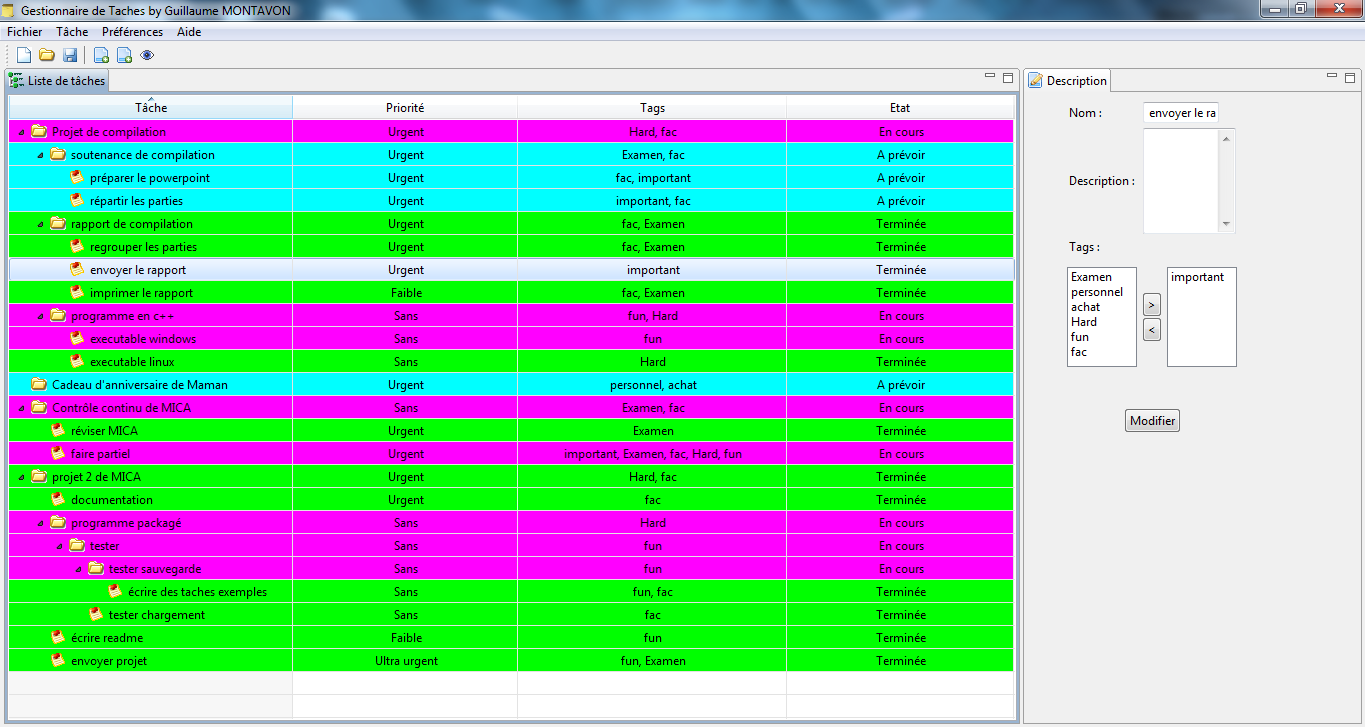
\includegraphics[width=13cm,height=8cm]{gestionnaireTacheExistantGuillaume.png}
        \caption{Example of screenshot of the existing task manager}

\end{figure}

\clearpage

\subsection{Presentation of the software for smartphones}

\noindent The sofware must be able to adapt to a smartphone while containing the functionnalities listed above. That is to say, he must be able to adapt to screen size, have a simple interface and not over-elaborate, but still full. It must also include new possibilities available with Android.


\section{Specifications}

\subsection{Application design}

\subsection{Technical constraints}

\subsection{Temporal constraints}


\clearpage
